% vim:ts=4:sw=4
% Copyright (c) 2014 Casper Ti. Vector
% Public domain.

\chapter{系统实现}
\section{爬虫模块}
基于在本文第二部分中的数据来源和爬虫的分析,采用beautifulSoup技术来进行爬取数据。
% \subsection{爬取基本数据}
\begin{figure}[h]
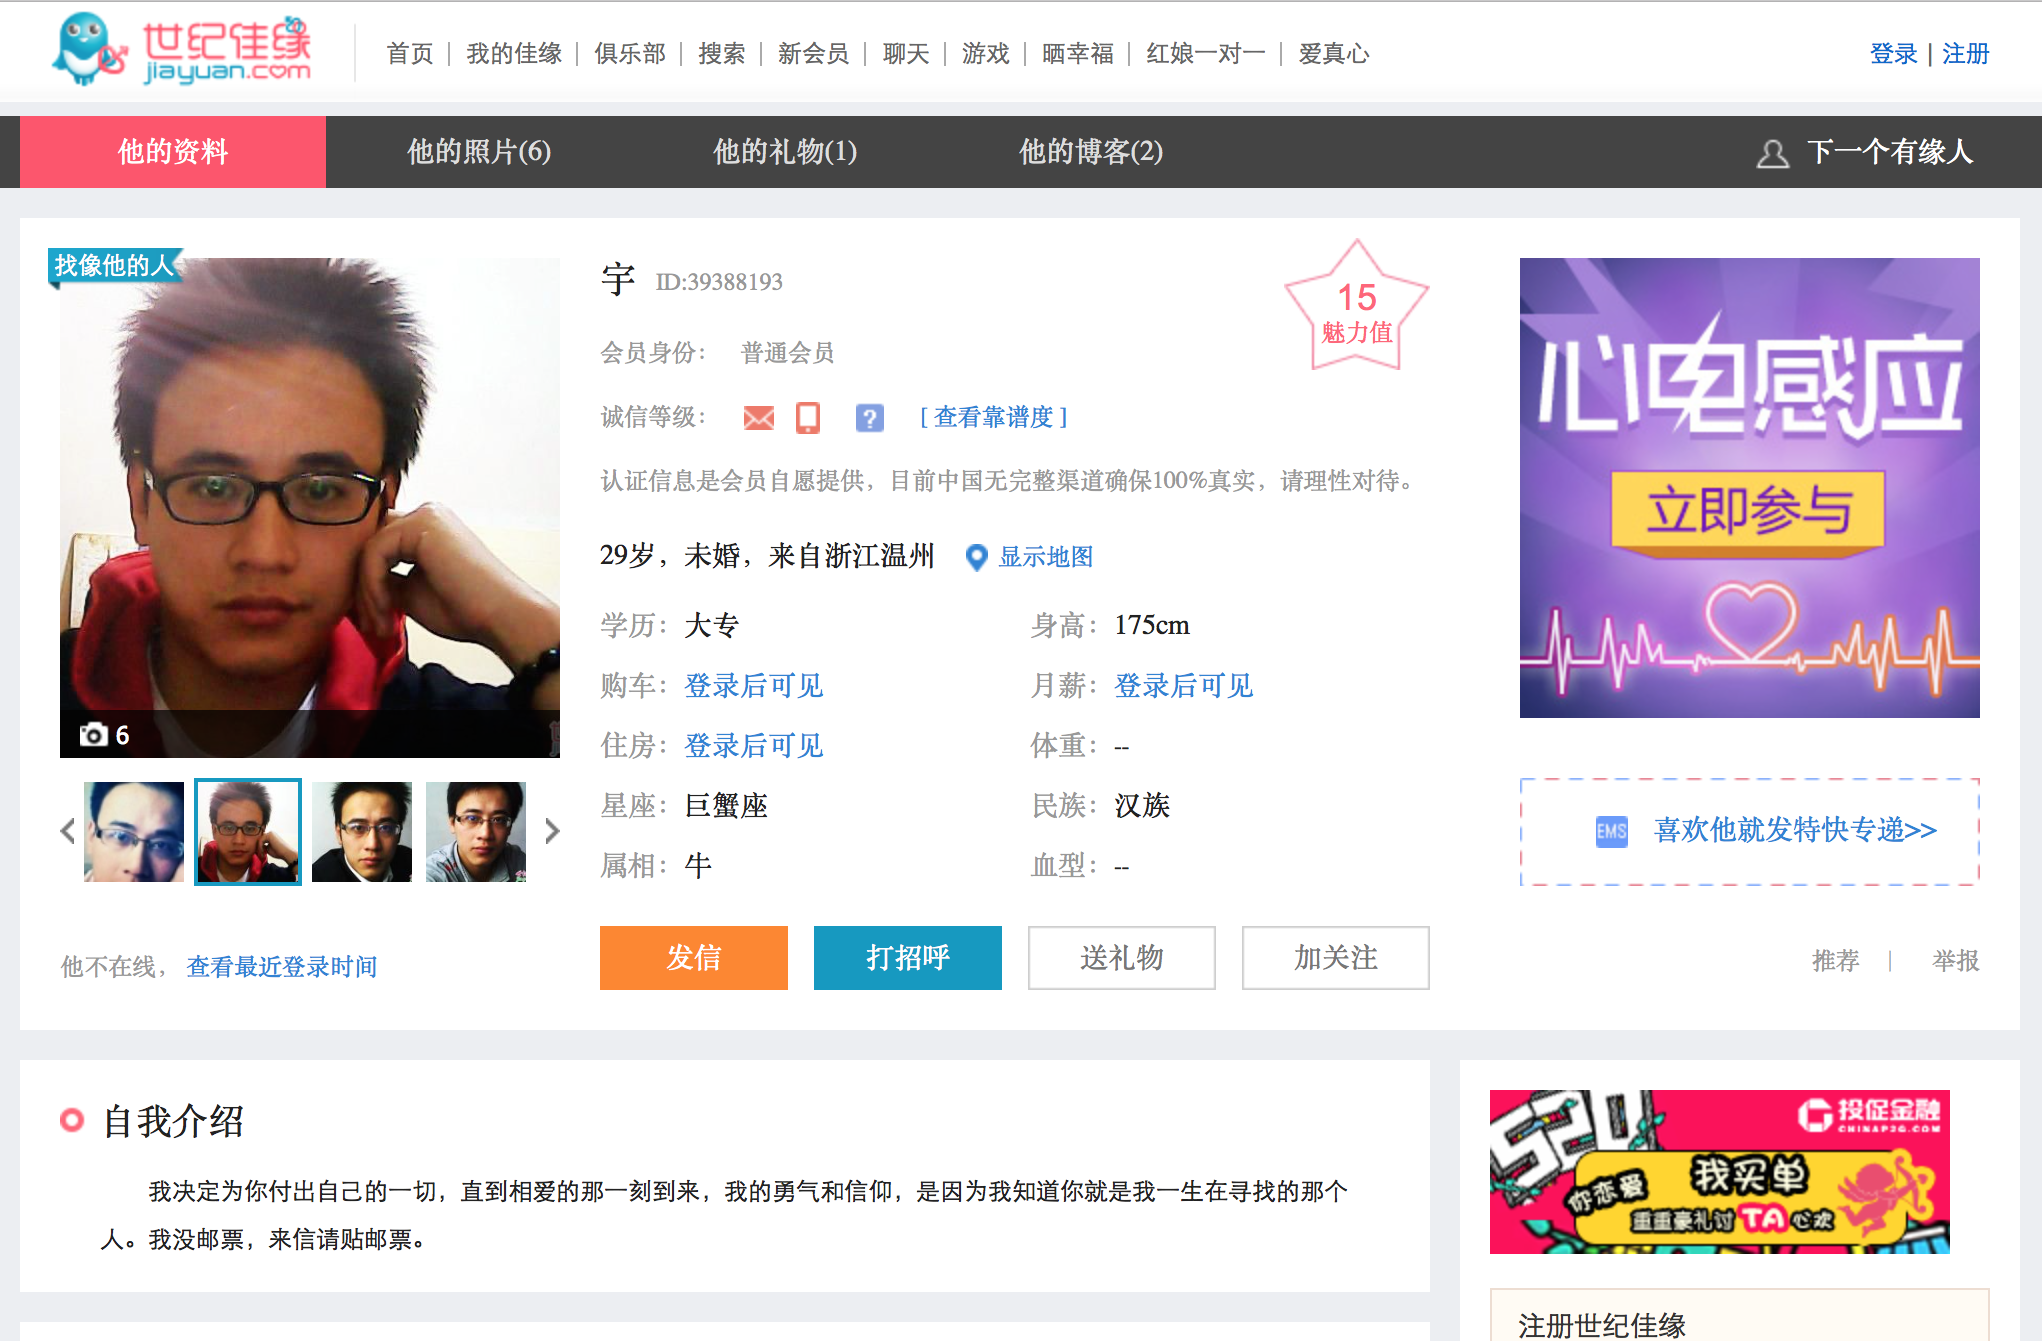
\includegraphics[width=\textwidth]{img/chap4/jiayuan1.png}
\caption{世纪佳缘用户信息页面\label{Face++API}}
\end{figure}
% \begin{figure}[h]
% 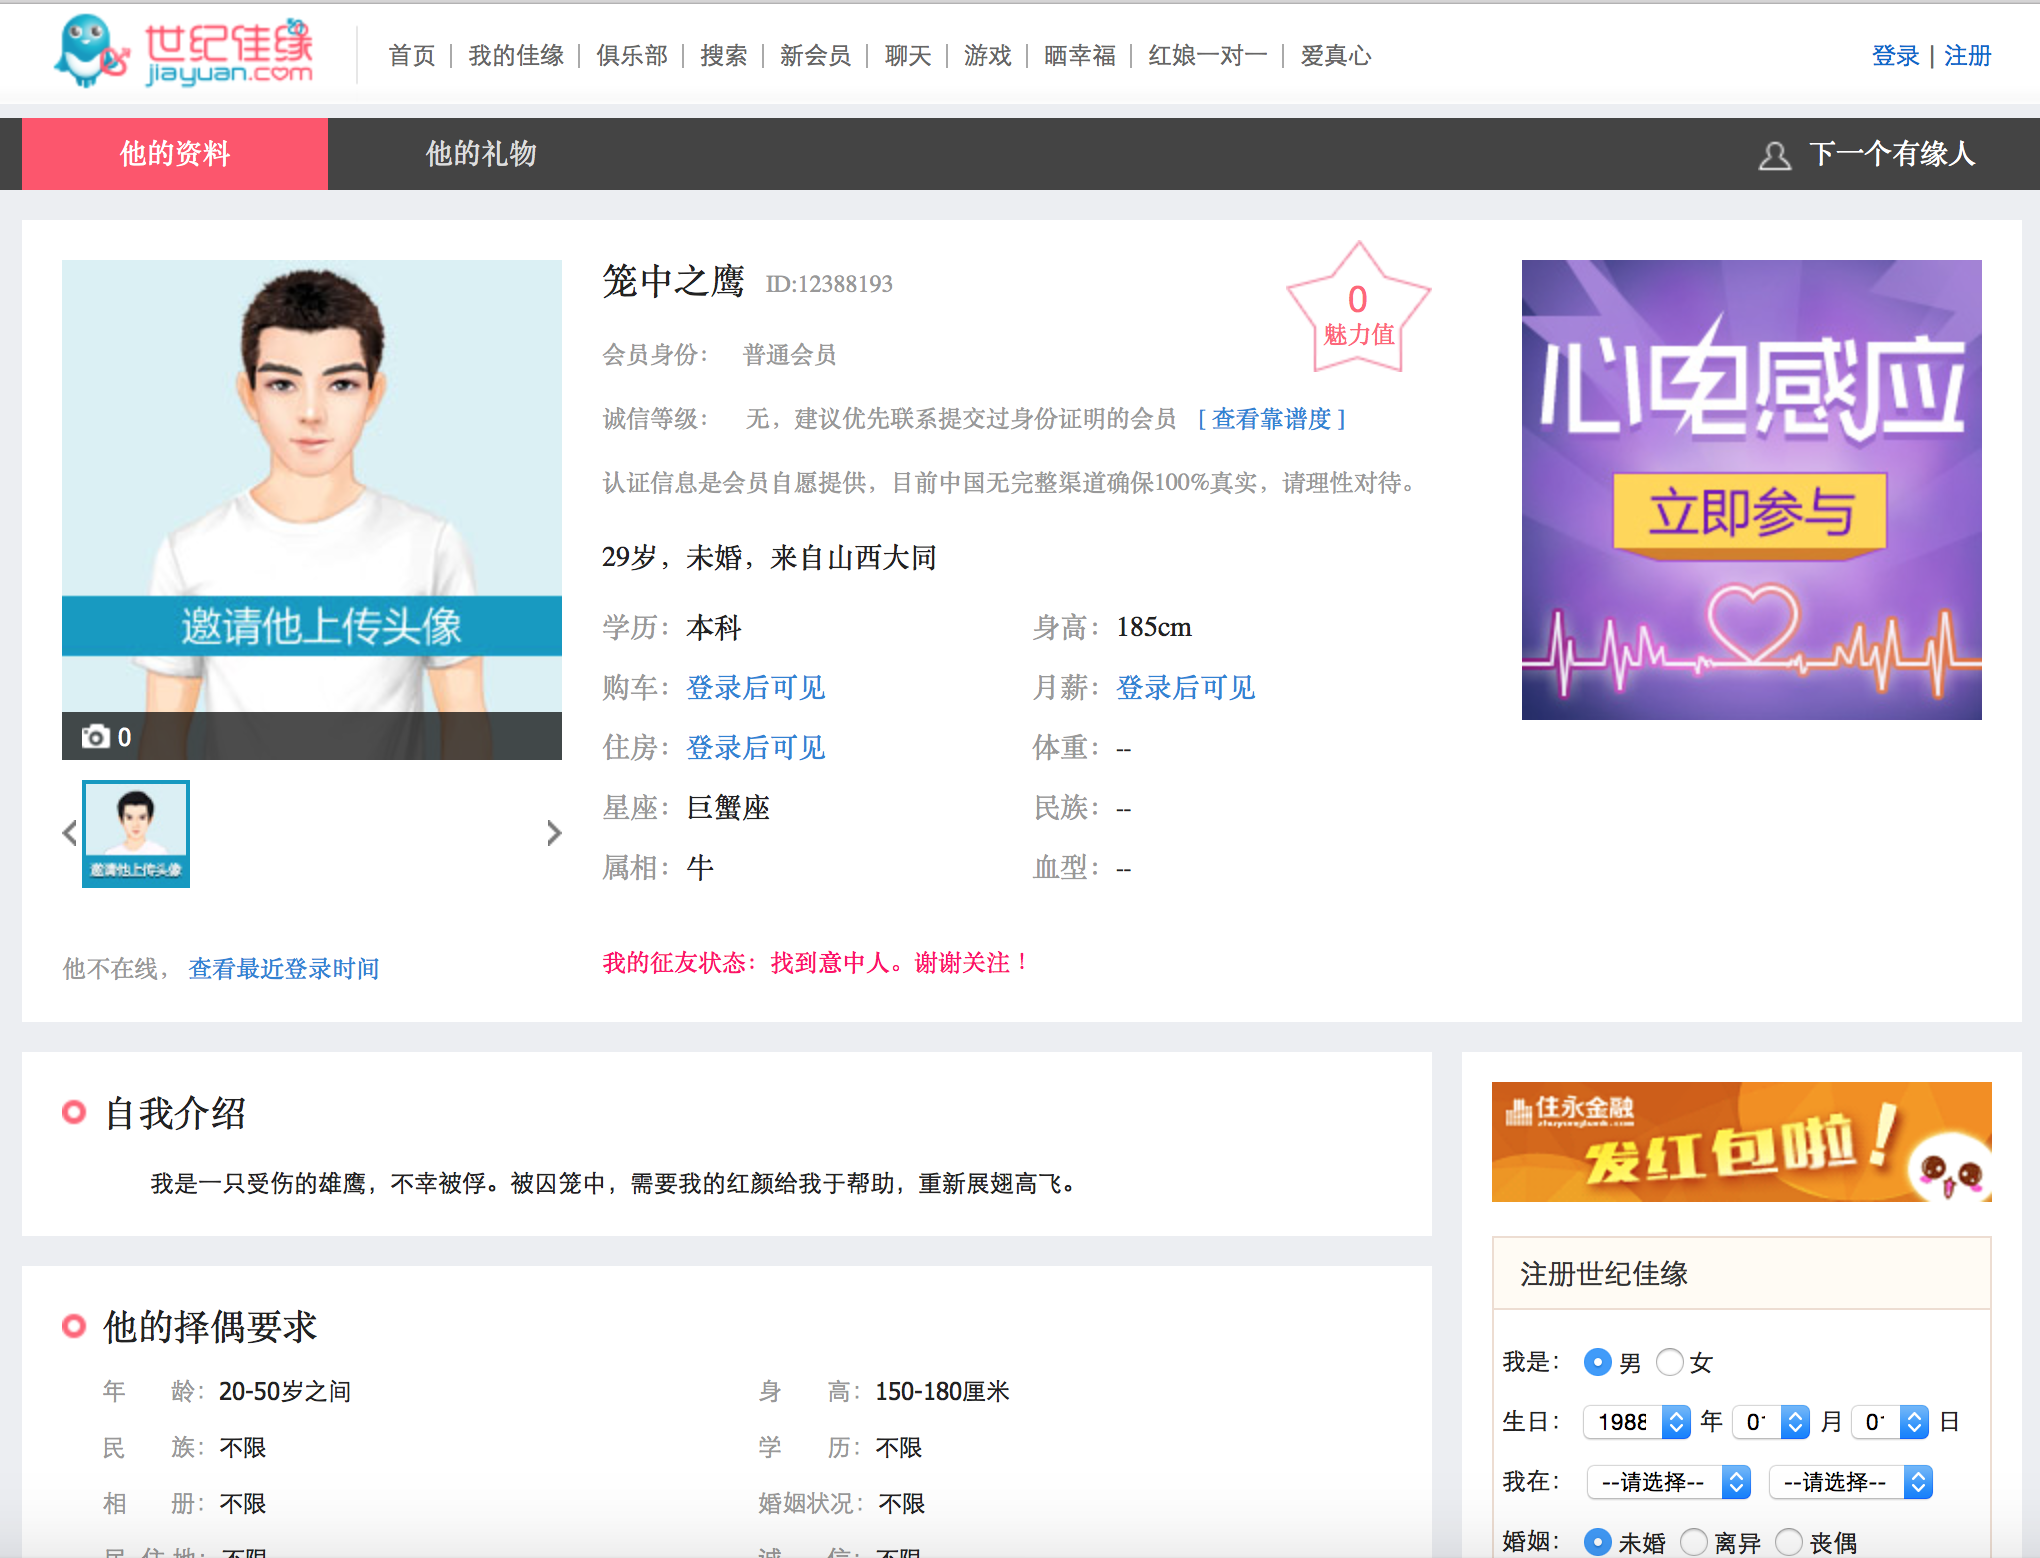
\includegraphics[width=\textwidth]{img/chap4/jiayuan2.png}
% \caption{世纪佳缘需权限信息页面\label{Face++API}}
% \end{figure}

通过前期充分对于世纪佳缘网站的调研,对于用户信息的分析,针对用户数据的发掘,本文找到了一个基于用户id以及对应用户数据联系的网页,从图4.1可以看出,此网页url可以连接到用户id具体的用户信息,从而我们可以针对指定的用户进行必要的信息的爬取。

但在实际操作中,一些用户的图片和信息设置为成权限可见之外,我们因此在程序中需要排除掉此类非法数据。除此之外其他的数据对于爬虫都是友好的,并且在一定程度上提供了丰富的用户信息,以便于我们进行匹配算法的优化。

最后我们的爬虫脚本对于抓取到的数据信息,存储到到本文的用户人脸数据库之中。

我们的爬虫的算法可以抽象成如下的伪代码。

\begin{codebox}
\Procname{$\proc{Crawler}$}
\li \For $j \gets $ \To the Amount of extrace \label{li:for}
\li     \Do \label{li:for-begin}
\li 	$URL \gets$ crawler url 
\li 	$Data \gets$ Raw data from $URL$
\li 	\For $k \gets$ Rule of Elements to form Data \label{li:for}
\li     	\Do \label{li:for-begin}
\li 		$info /gets$ information from $Data$ regulated by $k$
\li      	Insert $Info$ into the sorted sequence $Request$.
\label{li:for-end}
                \End
\li         Connect database submit $Request$ to database       \label{li:for-end}
        \End
\end{codebox}

该算法大致的思路如下:
\begin{itemize}
\item 确定爬取URL的个数
\item 循环,对于每个URL,从网页端爬取原始信息。
\item 对于每一个需求的信息的特征,进行不同的规则选取。
\item 对于特定的规则,在原始信息中提取特征信息
\item 将特征信息存入临时的表中
\item 连接数据库,将临时数据提交至数据库
\end{itemize}
% [伪代码1]
% \subsection{导入数据库}

% [伪代码2]

\section{应用端模块}
该应用的实现由三步组成:状态查询,信息源添加,和匹配反馈。


\subsection{状态查询及展示}
为了满足用户自己查询感兴趣好友的需求,应用需要提供用户在使⽤应⽤程序查看他人已经存在的Post信息。并为了便携性和可用性,需完成进行对于用户Post信息的一个预览,以及对于具体Post信息的查询。

从而可以满足用户的需求,去查看其他用户Post具体的信息,并可以支持用户随时对于需要的信息的刷新,以及链接用户更进一步的个人主页的途径。
\begin{figure}[h] 
\begin{minipage}[t]{0.3\linewidth}
\centering
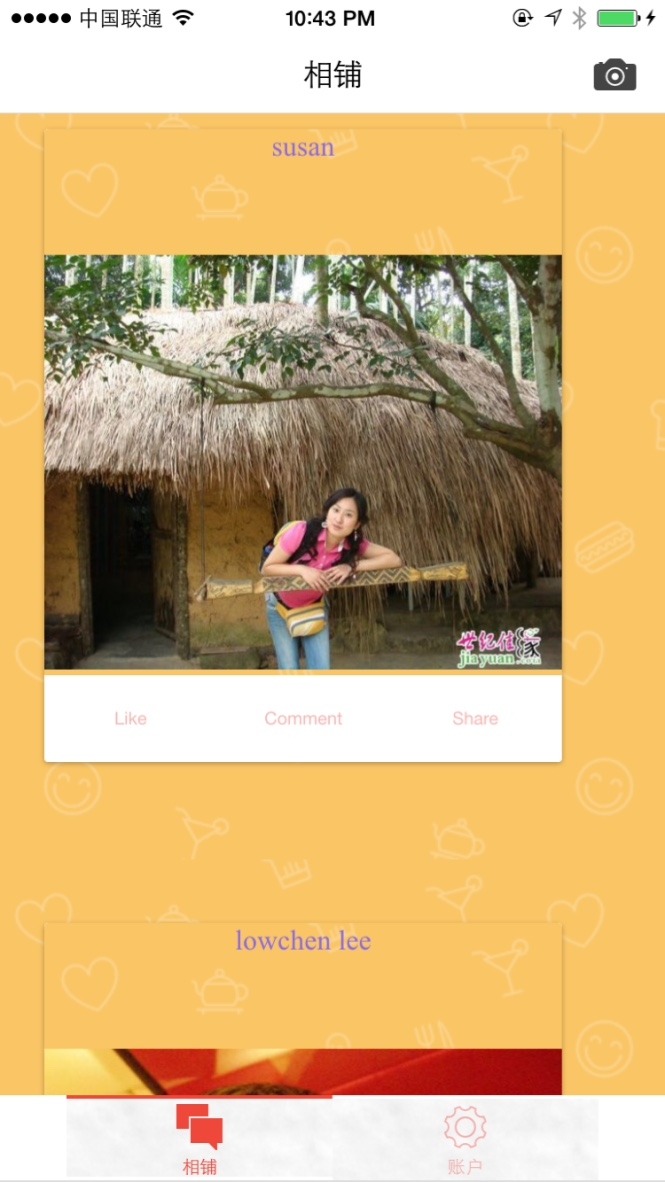
\includegraphics[width=\textwidth]{img/chap4/info1.jpg}
\caption{主界面\label{flickr}}
\end{minipage}
\hfill
\begin{minipage}[t]{0.3\linewidth}
\centering
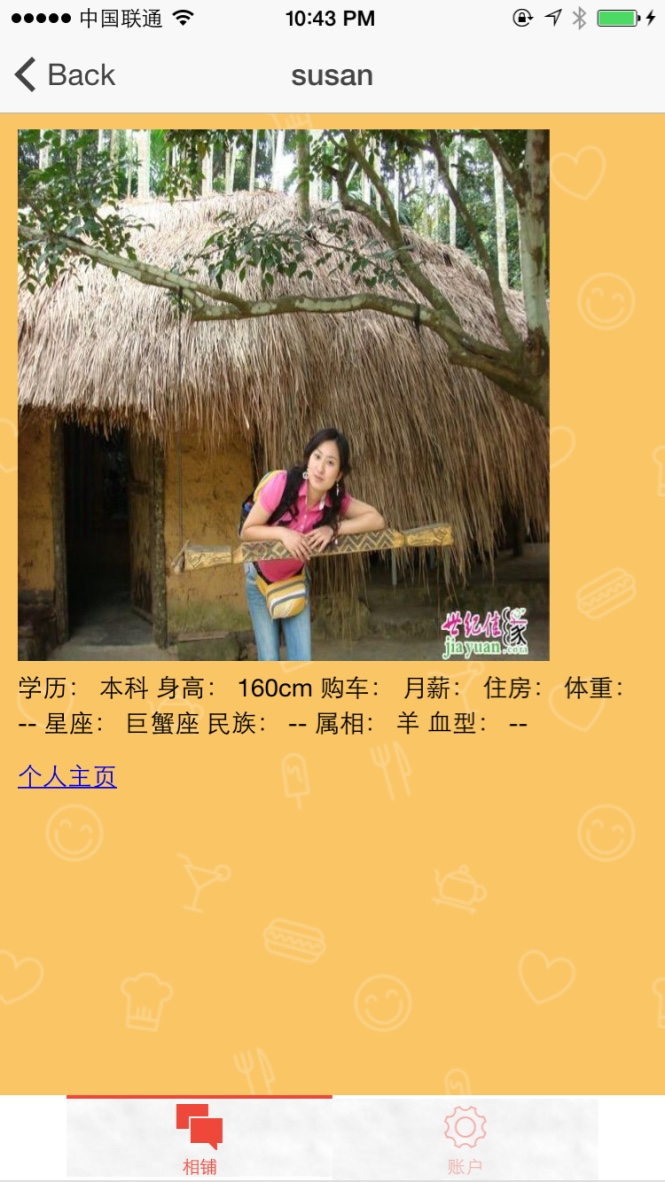
\includegraphics[width=\textwidth]{img/chap4/info2.jpg}
\caption{详细信息\label{instagram}}
\end{minipage}
\hfill
\begin{minipage}[t]{0.3\linewidth}
\centering
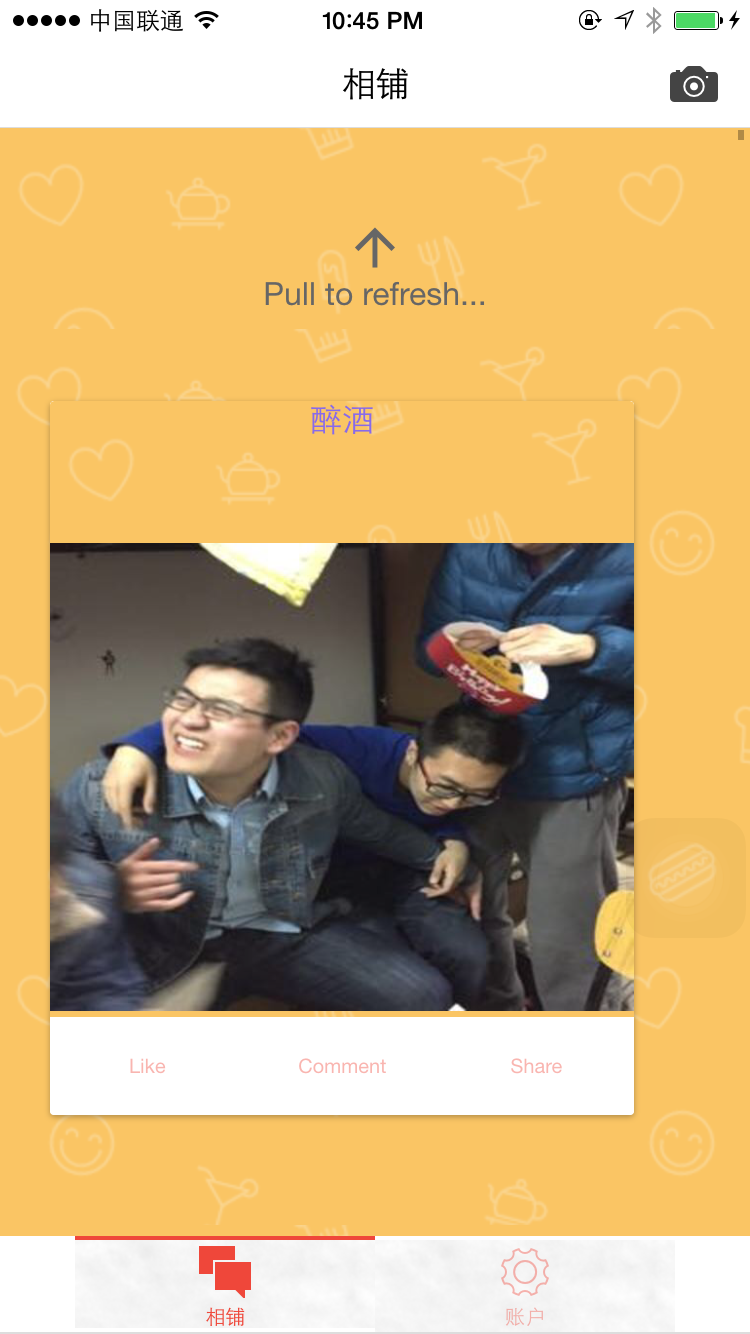
\includegraphics[width=\textwidth]{img/chap4/info3.PNG}
\caption{刷新\label{snapchat}}
\end{minipage}
\hfill
\end{figure}

进入应用,我们首先进入了主界面(图4.2所示),在这里我们可以看到用户Post的缩略图,既省略了用户的Post详细信息,可以达到快速浏览的目点,又为用户提供了一个可以找到自己兴趣点的信息。

如果对一个用户感兴趣,点击即可转到详细信息界面(图4.3所示),显示了用户Post的详细信息。

为了及时更新Post,主界面补充了刷新功能(图4.4所示),可以对主界面的Post进行刷新。

\subsection{信息源添加}
用户关于自己信息的发布通常希望其发布的信息具有多种多样的形式,考虑到移动设备较难编辑和显⽰富⽂本信息,应⽤用程序被实现为能够编辑、存储和显示具有多种类型的字段,包括个人姓名、个人介绍、URL和提交的匹配图片

并且基于用户照片来源的不同,分为从用户的图片库中采集和即时照相两种不同图片来源方式。并在此基础上实现了图片预览的功能。
\begin{figure}[h] 
\begin{minipage}[t]{0.3\linewidth}
\centering
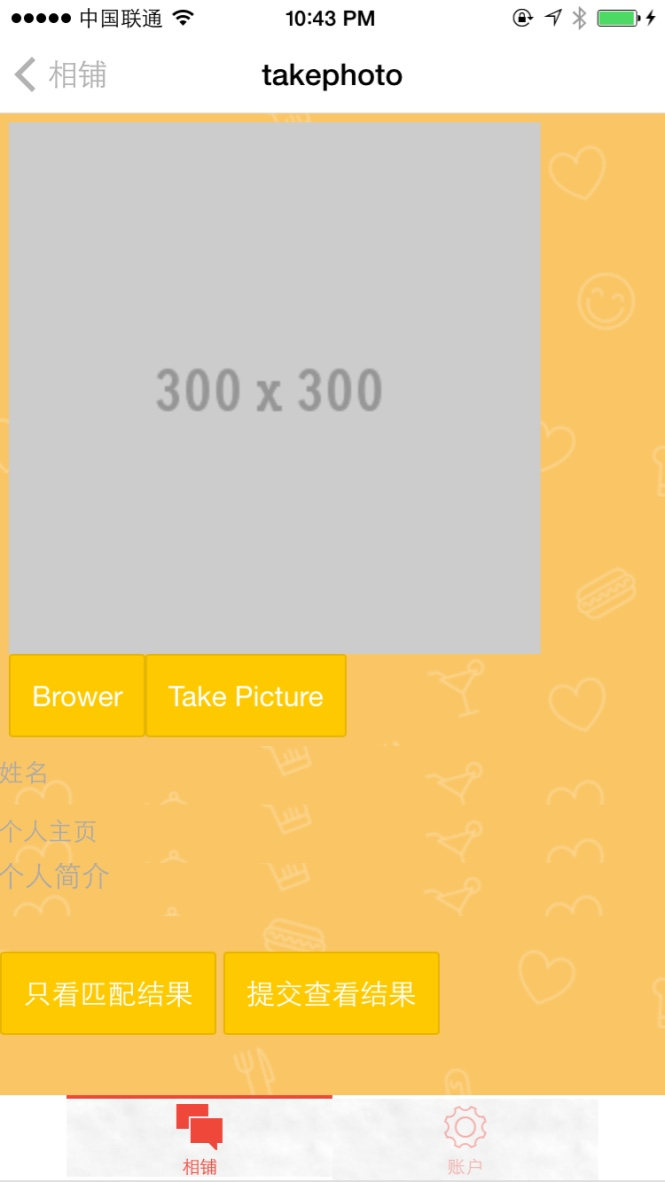
\includegraphics[width=\textwidth]{img/chap4/take1.jpg}
\caption{提交界面\label{flickr}}
\end{minipage}
\hfill
\begin{minipage}[t]{0.3\linewidth}
\centering
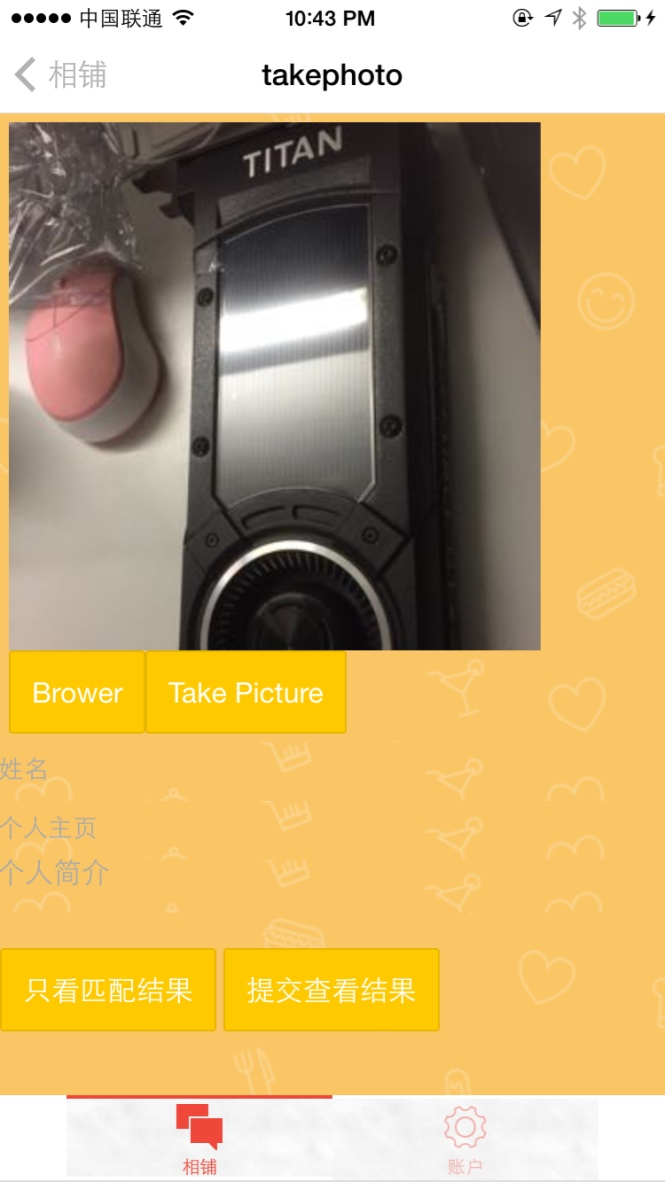
\includegraphics[width=\textwidth]{img/chap4/take2.jpg}
\caption{预览提交的图片\label{instagram}}
\end{minipage}
\hfill
\begin{minipage}[t]{0.3\linewidth}
\centering
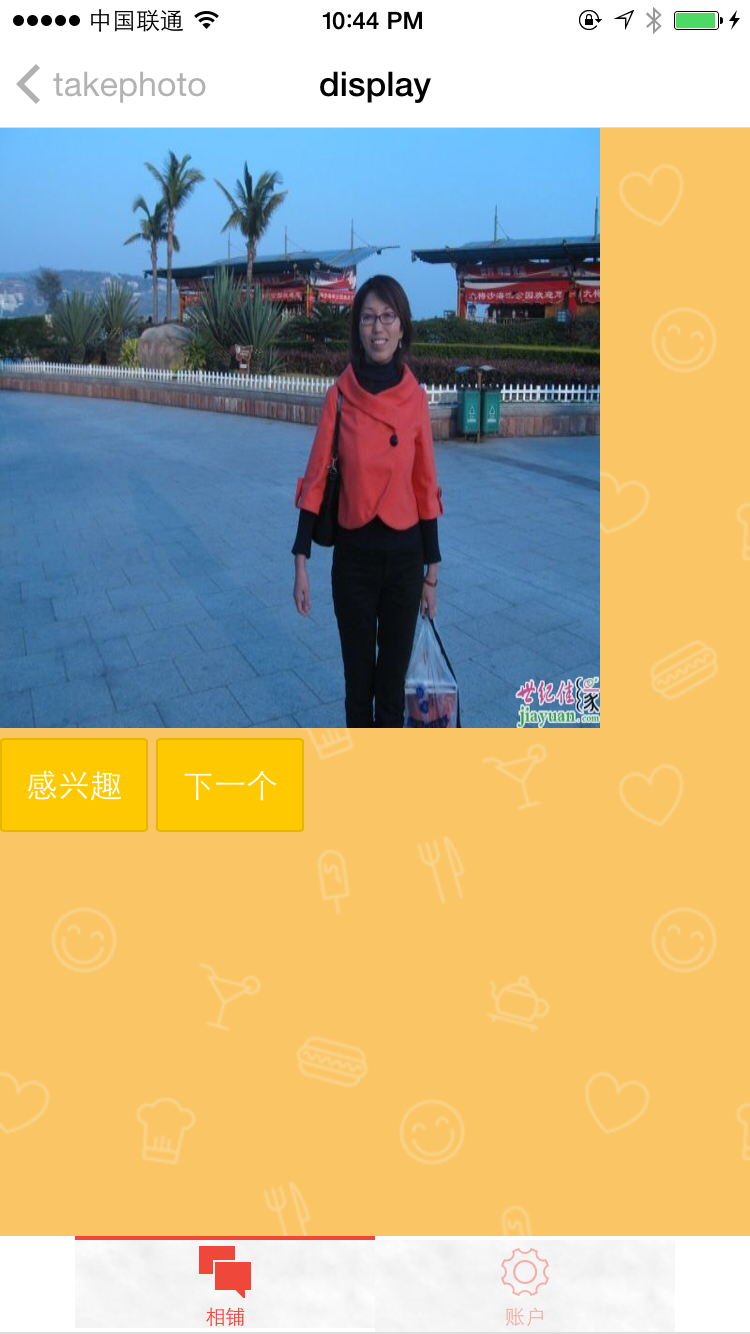
\includegraphics[width=\textwidth]{img/chap4/display.PNG}
\caption{展示界面\label{instagram}}
\end{minipage}



\end{figure}
图4.5和4.6展示了这两项功能,提供用户描述自己Post信息的通道,并使得用户能够通过不同的方式提供自己的人脸图片,并预览自己提交的图片。
\subsection{匹配信息展⽰}
由于服务端有客户端提交的图片以及文本信息直接调用对应匹配算法的接口,因此,应用端在用户在提交了自己的信息之后可以直接调用了此接口,服务端便具有了足够的信息以匹配出对应的好友。

在服务端返回给客户端匹配出的结果后,客户端将详细信息显⽰在⽤用户界⾯上(图4.7所示)。这里具有具有多条匹配结果,客户端将按照匹配程度顺序将结果显⽰。当用户对该用户感兴趣时即点击“感兴趣”按钮进入查询详细信息。




